
\chapter{Глава 5}

Вновь желаю здравствовать своим читателям. С вами снова серия, посвящённая стратегическому выбору направления экспансии Страны Восходящего солнца.

Что ж, в прошлый раз мы достаточно подробно разобрались с китайскими делами – без сомнения, высшим приоритетом для Японии в период 1914-1918. Вновь поговорили мы и о власти, о тех органах и тех конкретных людях, которые принимали ключевые решения. Ну а в завершении подошли к вопросу об участии Японии в интервенции в России и последствиях для неё такого шага. Но, прежде чем переходить к этой теме, стоит немного сказать о развитии отношений России и Японии после Русско-японской войны вообще. Для России годы, последовавшие за Портсмутским миром, принесли не просто переориентацию с Дальнего Востока обратно на Европу, но и быстрое ускорение и углубление вовлеченности в имевшийся там клубок противоречий. В 1908 разгорелся Боснийский кризис, который легко мог привести к войне (собственно, по общему мнению и современников, и нынешних исследователей аннексия Боснии Австро-Венгрией как повод к войне была куда весомее Сараевского убийства и его прямых последствий). Параллельно в 1906 и 1907 годах продолжала бушевать Первая русская революция, причём всё более, так сказать, уходя на низовой, наиболее сложный для купирования уровень массовых и повсеместных крестьянских выступлений. Военные долги и общий социально-экономический разлад заставляли всё более активно обращаться к внешним заимствованиям, прежде всего у союзников-французов. Так же Франция и её капитал вообще всё активнее проникали в нашу экономику и промышленность, что в свою очередь увеличивало степень зависимости от её воли при принятии решений. Французов же слабо интересовал Дальний Восток, но очень живо – Германия и противодействие ей. Схожие интересы у ведущей дредноутную гонку и торгово-экономическую борьбу со Вторым рейхом Британии. И вот 1907 год становится моментом, когда тянувшаяся большую часть XIX столетия Большая игра и Русско-английский антагонизм должны были отойти на второй план перед лицом перемен. В августе было подписано Русско-английское соглашение по разграничению сфер влияния в Персии, а также окончательному закреплению статуса Афганистана и Тибета. Разумеется, британский союзник – Япония не могла не учитывать этого факта.

Вообще с японской стороны, о чём уже говорилось в предыдущих частях, существовало понимание, что без большой войны с России ничего получить не удастся, а таковая война вполне может окончиться для Японии гибелью, так как совершенно неясно каким способом принуждать Российскую Империю к миру, затяжной же конфликт вёл в целому ряду очень серьёзных рисков, как военного, так и экономического плана. Наиболее мудрые государственные мужи Империи Восходящего солнца – и в первую очередь самый авторитетный из Гэнро – Ито Хиробуми, определённо выступали за мирные отношения с Россией и даже сотрудничество с ней, при условии признания Петербургом не только гласных результатов Русско-японской войны, закреплённых в мирном договоре, но и негласных, так сказать, подразумевавшихся. В первую очередь, окончательного и полного перехода Кореи под власть Японии. Именно об этом и велись переговоры между Хиробуми и Коковцовым в 1909 Харбине и, несмотря на то, что великий японский государственный деятель, как мы помним, был убит (что стало для страны потерей, сравнимой со смертью в 1912 самого Мэйдзи), стороны пришли к пониманию.

Ну а в 1914 грянула Первая мировая. Как только позиция Японии в августе 1914 вполне прояснилась с её ультиматумом Германии, 24 числа туда из России выехала военно-техническая комиссия во главе с генерал-майором Э. К. Гермониусом. Первоначальной задачей комиссии было приобретение в Японии запаса трофейных трехлинейных винтовок, захваченных японской армией в ходе русско-японской войны. В сентябре 1914 года японские власти сообщили, что запасы трёхлинейных винтовок уже утилизированы. Тут бы и конец, но японцы предложили закупить вместо этого 35 000 винтовок и карабинов «Арисака», изготовленных по заказу правительства Мексики, и 23 миллиона патронов к ним. 

\begin{figure}[h!tb] 
	\centering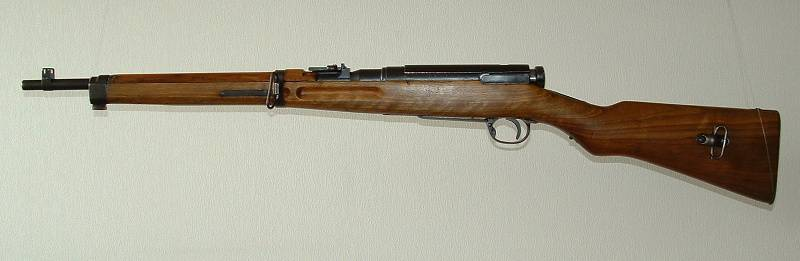
\includegraphics[scale=0.4]{Glava5/aPLBzctcRUE.jpg}
	%	\label{fig:scipion} % Unique label used for referencing the figure in-text\end{document}
	%	%\addcontentsline{toc}{figure}{Figure \ref{fig:placeholder}} % Uncomment to add the figure to the table of contents%----------------------------------------------------------------------------------------
	\caption{Винтовка Арисака Тип-38}%	CHAPTER 2
\end{figure}

Партия, на самом деле, весьма скромная. Основной причиной предложения японцев было их собственное желание избавиться от экспортной версии Арисаки, так как её патроны не подходили не только ни к немецким, ни к русским винтовкам, калибр которых был больше, чем принятые в Японии 6,5 мм, но даже и к своим, японским винтовкам в стандартном их варианте. 13 октября 1914 года 20 350 винтовок, 15050 карабинов и патроны были куплены за 200 тыс. фунтов стерлингов, т.е. около 2 миллионов золотых рублей по курсу 1914 года. Но и это был далеко не конец.

Напротив, вслед за этим, Гермониус получил приказ закупить ещё «до миллиона(!) винтовок японской армии с запасом 1000 патронов на каждую винтовку». Недурственный скачок с 35 000! Заказ был столь неожиданным, что его без особенного энтузиазма восприняла даже японская армия, рисковавшая сильно сократить свой арсенал, но после переговоров она всё же согласилась продать 200 000 уже снятых с вооружения винтовок обр.1897 года и 25 млн патронов к ним (125 шт. на винтовку). Причём японцы даже честно предупредили, что патроны будут старые, с истёкшим сроком годности, со складов в Корее. Тем не менее, уже 21 октября 1914 года в огромной спешке был подписан контракт на поставку оговорённого количества винтовок и патронов за 4,5 млн золотых рублей. Автор не является специалистом в этой области, но не может не отметить, что всё это выглядит чрезвычайно подозрительно – комиссия, посланная с конкретной и весьма скромной с точки зрения затрат задачей в итоге заключает совершенно другие, а главное миллионные сделки и в самые короткие сроки. Есть немалое подозрение, что во всём этом была, как сейчас бы сказали, “коррупционная составляющая в сфере госзакупок и оборонного заказа”.

Торговля изношенными и малопригодными винтовками продолжалась и далее. В январе 1915 года на официальный запрос о продаже ещё 300 000 винтовок японское правительство, не желавшее сокращать мобилизационный резерв, согласилось продать лишь 100 000 самых изношенных винтовок старого образца. 28 января 1915 года был подписан контракт на поставку 85 000 винтовок, 15 000 карабинов и 22,6 миллионов патронов (на общую сумму 2 612 000 иен или около 2,5 миллионов рублей), а 3 февраля 1915 года — ещё 10 миллионов патронов к ним. Японцы достаточно быстро ощутили свою выгоду и стали умело пользоваться сложившимся положением. Русским нужны винтовки? Прекрасно! 25 мая 1915 года в обмен на политическую поддержку Россией японского ультиматума к правительству Китая, Япония согласилась продать ещё 100 000 винтовок и 20 миллионов патронов, в начале сентября 1915 года — продала ещё 150 000 винтовок нового образца «тип 38» и 84 миллиона патронов. Оба контракта были оплачены золотом. Иными словами, японцы разом и решали важную политическую задачу – Россия в год Великого отступления едва ли могла помешать японцам давить на Китай, но её неодобрение могло сказать в будущем, и получали немалую материальную выгоду, да ещё и обставляла всё это как уступку.

Если подсчитать общую сумму, то выходит, что Россия закупила за полтора года (напомню, строго за золото) 585 000 винтовок и карабинов Арисака, но даже и это оказывается не полной величиной. Ещё 128 000 штук было получено в 1916 году не прямо от Японии, а из Великобритании, некоторое количество винтовок было из китайского и мексиканского заказов («мексиканские карабины», например, использовались пограничниками и Заамурским военным округом). Нельзя сказать, чтобы винтовка так уж активно применялась на Русско-германском фронте, но в целом она была до такой степени “освоена” Россией, что именно под её патрон конструктор Фёдоров разработал свой ныне знаменитый автомат.

Вообще не следует думать, что со стороны Империи Восходящего солнца имел место некий злонамеренный обман: Арисака была вполне удачной винтовкой, а японцы честно исполняли свои обязательства. Инициатива в вопросе о закупках исходила именно от российской стороны, а у японцев не было никаких мотивов, чтобы не извлечь из этого всю выгоду. В целом отношения с Российской Империей в 1914-1917 нельзя назвать дружескими, но вполне можно конструктивными. Японцы даже (хотя, надо думать, и не без собственных видов), одобрили подписание Кяхтинского договора 1915, согласно которому официально Монголия (тогда Внешняя Монголия) обретала законодательно закреплённую автономию в рамках Китая, а фактически превращалась в полунезависимое государство под русским протекторатом. Февраль 1917 мало что изменил – в первую очередь, вероятно, потому, что японцы, как и многие другие, не заметили всего масштаба перемен, которые стали происходить в России. Главным образом это произошло из-за того, что отречение царя было воспринято со всеобщим одобрением – ни одна социальная прослойка, ни одна страна, класс, группа влияния, буквально никто, даже в императорской фамилии (о чём очень бы хорошо помнить нынешним любителям похрустеть французской булкой) не только не попытался отстоять власть Николая II, но даже не выразил сожаления в связи с его уходом.

Конечно же, всё изменилось к концу лета 1917, когда такие вещи, как Корниловский мятеж, уже нельзя было не заметить. Ну а окончательно события перешли в галоп после Октябрьской революции и опубликования Декрета о мире. Стали очевидными две вещи:

1) Русские собираются выйти из войны.

2) Россия переживает серьёзный внутренний кризис

Разумеется, весьма быстро стали возникать планы относительно того, как этим можно воспользоваться. Впрочем, изначально Япония не пыталась бежать впереди паровоза. Ещё не был заключен Брестский мир, даже переговоры ещё не начинались, так что формально Россия продолжала оставаться союзником Империи Восходящего солнца. И вообще было совершенно очевидно, что возникший вдруг русский вопрос Антанта будет решать комплексно и с участием всех ключевых держав. 3 декабря 1917 года собралась специальная конференция с участием США, Великобритании, Франции и союзных им стран, на которой было принято решение о разграничении зон интересов на территориях бывшей Российской империи и установлении контактов с национально-демократическими правительствами. К слову сказать, Гражданская война в это время в целом ещё не началась, спорадические бои, имевшие место непосредственно в октябре 1917, окончились, за значимым, но совершенно особенным по своему генезису исключением Украинской Центральной Рады, вся страна признала власть Советского правительства, так что господа из Антанты нагло и явно вмешивались в суверенные дела России из своих корыстных интересов и активно искали себе в этом деле помощников.

Ключевым был вопрос о войсках. Всем было понятно, что большевики – не из тех, кто испугается давления, ну а в самой критической ситуации они могли обратиться за помощью и к Германии. Это означало, что при организации интервенции нужно или сразу задействовать большое количество сил и средств, чтобы уверено повалить Советы, или минимизировать масштабы интервенции, создать иллюзию, что вмешательство осуществляется исключительно по отдельным, частным вопросам, как то охрана военных складов, транзит и вывод союзнических частей, уже находящихся на русских территориях, но не покушается на самостоятельность и проводимый курс России. Первый вариант, весьма заманчивый, практически был малореален, так как почти все наличные силы Англии и Франции были задействованы на фронтах. Соединённые Штаты были перегружены логистически – даже их транспортного флота не хватало одновременно на то, чтобы перебрасывать сотни тысяч бойцов и массы грузов и во французские порты, и в Россию. Весьма неожиданно оказалось, что именно Япония из всех союзников обладает наиболее крупными, свободными и близко расположенными к российским пределам силами. Правда, значительно удалёнными от Петрограда и от разваливающегося Русско-германского фронта.

Начало было положено 12 января 1918 год, когда японский крейсер «Ивами» вошёл в бухту Владивостока для «защиты интересов и жизни проживающих на российской земле японских подданных», при этом утверждалось, что японское правительство не намерено «вмешиваться в вопрос о политическом устройстве России». Несколько дней спустя во Владивосток прибыли военные корабли США и Китая. В общем, это сложно ещё назвать интервенцией в полном смысле слова – скорее это было обозначение присутствия. Оно ни к чему не обязывало, не требовало затрат, но и ни к чему не вело.

Ещё в конце 1917 года Франция, которая была слабо заинтересована в Дальнем Востоке, предложила по дипломатическим каналам японцам войти на территорию Приморья и даже Сибири. Япония отказалась. Причин тому много. Главная, пожалуй, это то, что предложение исходило от одной только Франции – до тех пор, пока позиция других держав Антанты не была вполне прояснена, делать излишне резкие шаги было неосмотрительно. Кроме этого, Россия всё ещё не выглядела раскалывающимся на части сосудом – власть большевиков казалась почти общепризнанной и способной организовать серьёзное вооружённое сопротивление. Наконец, в отличие от реально сражавшихся в ПМВ государств, Япония ещё не была вполне готова с точки зрения мобилизации вооруженных сил и, особенно, промышленности к отправке крупного воинского контингента. Пока что японцы хотели получить пусть не столько много, но зато без особенных трат и надёжно. 18 февраля 1918 года Верховный совет Антанты – разумеется, с подачи Империи Восходящего солнца, принял решение об оккупации японскими войсками Харбина, а также зоны КВЖД, т.е. территорий, России принадлежавших, но не являвшихся прямо её частями. Одновременно решена была и судьба Владивостока, куда предполагалось направить уже объединённые силы под предлогом охраны ввезённых военных материалов. И Харбин и КВЖД были весьма ценными приобретениями, но только не одни лишь японцы понимали это. В конце февраля – начале марта 1918 интервенция стала уже решенным делом – переговоры в Бресте между РСФСР и Центральными державами вступили в заключительную фазу и стало понятно, что Россия окажется вынужденной многое уступить Германии и её союзникам. Японцы, без сомнения, должны были оказаться в числе основных участников. И, в рамках предварительных обсуждений будущих действий союзников в России, США, опасавшиеся чрезмерного усиления Японии в северо-западной части Тихого океана, потребовали от неё обязательства не предпринимать широких операций без ведома и согласия Антанты, а также вывести свои войска после достижения целей интервенции.

Руководители Империи Восходящего солнца встали перед весьма нелёгким выбором. С одной стороны Штаты просто предлагали Японии таскать каштаны из огня, не обещая ничего взамен: для японцев вопрос о власти в России и о том, будет или нет, эта власть дальше воевать с Германией был совершенно непринципиален. Япония свою Первую мировую по существу окончила ещё взятием Циндао, да и примкнула к Антанте исключительно исходя из своих интересов. Перемены на европейских фронтах волновали Страну Восходящего солнца довольно слабо. С другой стороны, японцы понимали – союзники нуждаются сейчас в них куда больше, чем они в союзниках. Свободные и пригодные войска кроме Японии, предоставить некому. США перед входом японцев в большую игру Интервенции требуют от них принять определённый свод правил – что ж, пусть так. Какое это имеет значение, если потом, когда десятки тысяч солдат под белыми флагами с красным кругом уже будут на месте, они не сумеют заставить Японию эти правила выполнять?

Другое дело, что попытка повести самостоятельную линию в России и проигнорировать договорённости со Штатами могла аукнуться потом, когда война закончится, и победители будут предъявлять ранее не столь актуальные, по сравнению с задачей одержать победу над врагом, счета друг другу. И в первую очередь в Китае, где и так был риск того, что двусторонние договорённости 1915 года и 13 принятых Пекином пунктов могут быть пересмотрены. Требовалось так быстро и так прочно встать в Приморье и вообще на Дальнем Востоке России, чтобы до окончания войны уже продавить и формально закрепить в Верховном Совете Антанты выгодные Стране Восходящего солнца территориально-политические изменения. Исходя из того, что происходило в марте 1918 во Франции, где немецкие войска готовили самое масштабное с 1914 наступление, а вернее даже целую серию ударов, спланированных Людендорфом, чтобы раскачать и обвалить фронт, японцы как будто могли рассчитывать на то, что война завершится ещё не скоро. Всё равно, однако, у замысла масштабного участия Японии в Интервенции были и свои противники. Во-первых, многие полагали, что риски утратить то, что с таким трудом было приобретено в Китае, будут слишком большими, и не следует распылять силы на что-либо ещё. Китай, завоевание доминирующего положения в нём, был целью всей политики страны с 1914 года (а по существу и с более ранних времен), и теперь нельзя было просто временно отложить его в сторону. Во-вторых, по-настоящему мощные экспедиционные силы требовали и весомых затрат, а экономика и бюджет Страны Восходящего солнца не были готовы к дополнительным крупным расходам. Наконец, по-прежнему было неясно с какой силы сопротивлением придётся столкнуться войскам, и какие они могут понести потери. Одним словом, аргументы у противников Интервенции были довольно серьёзными – в итоге дело дойдёт даже до совершенно непривычно острых по меркам Японии дебатов в парламенте. Но только будет это уже летом 1918, когда истинный масштаб задуманного стал всем понятен. В марте же 1918, когда всё только начиналось, решение, судя по всему, было принято или единолично премьером Масатакэ, или небольшой группой близких к нему людей – в основном военной закалки.

Действительно, с чисто военной точки зрения всё выглядело довольно просто, а обещало много. Тераути Мастакэ всегда был человеком решительным, способным без колебаний и отклонений, «брать штурмом» ту или иную задачу, а теперь, по-видимому, воспринимал своё назначение главой кабинета в октябре 1916 с той точки зрения, что именно это качество, по мнению людей, способствовавших его продвижению, и требуется. И вот 16 марта 1918 японское правительство дало американцам требуемые заверения. Теперь нужен был повод – его нашли очень быстро. 4 апреля 1918 года во Владивостоке были убиты двое японских служащих коммерческой компании. На следующий день, не дожидаясь расследования дела, японцы высадили в город десант под предлогом защиты японских подданных, некоторое время спустя вслед за японцами высадились и англичане. Но основные события развернулись 29 июня 1918 года, когда с помощью восставших чехословаков во Владивостоке была свергнута советская власть.

Вообще Чехословацкий мятеж переменил очень многое. Большевики разом утратили контроль над большой частью России – и все их противники одновременно не преминули этим воспользоваться. В стране началась большая и страшная Гражданская война. А за границей 2 июля 1918 года Верховный военный совет Антанты принял решение расширить масштабы интервенции в Сибири. Президент США Вудро Вильсон уже гласно и открыто попросил Японскую империю о выделении 7 тысяч человек в состав 25-тысячного международного контингента, официально предназначенного для помощи в эвакуации с российской территории чехословацкого корпуса. Вот тут и пришло, запоздало, время для бурных дебатов в парламенте Японии. Премьер Масатакэ действовал быстро и бескомпромиссно и здесь – не обращая внимания на парламентариев, рассчитывая (как оказалось, справедливо), что сумеет их дожать, он начинает торг со Штатами. Вместо 7 000 он готов дать сразу 12 000, но при условии, что японский контингент не будет частью международных сил, а получит собственное командование. Или – ничего. Тут как раз пригодились видимые признаки оппозиции в Стране Восходящего солнца участию в интервенции. И США пасуют! Согласие Вильсона получено. Далее всё начинает идти в строгом соответствии с планом – Япония плюёт на любые ограничения, бешеными темпами наращивает своё присутствие - к октябрю 1918 года численность японских войск в России достигла 72 тысяч человек (в то время как американский экспедиционный корпус насчитывал 10 тысяч человек, а войска других стран — 28 тысяч человек). И эти части не сидят без дела – в короткий срок и, как оказалось, при минимальном противодействии, они оккупировали Приморье, Приамурье и Забайкалье. 

\begin{figure}[h!tb] 
	\centering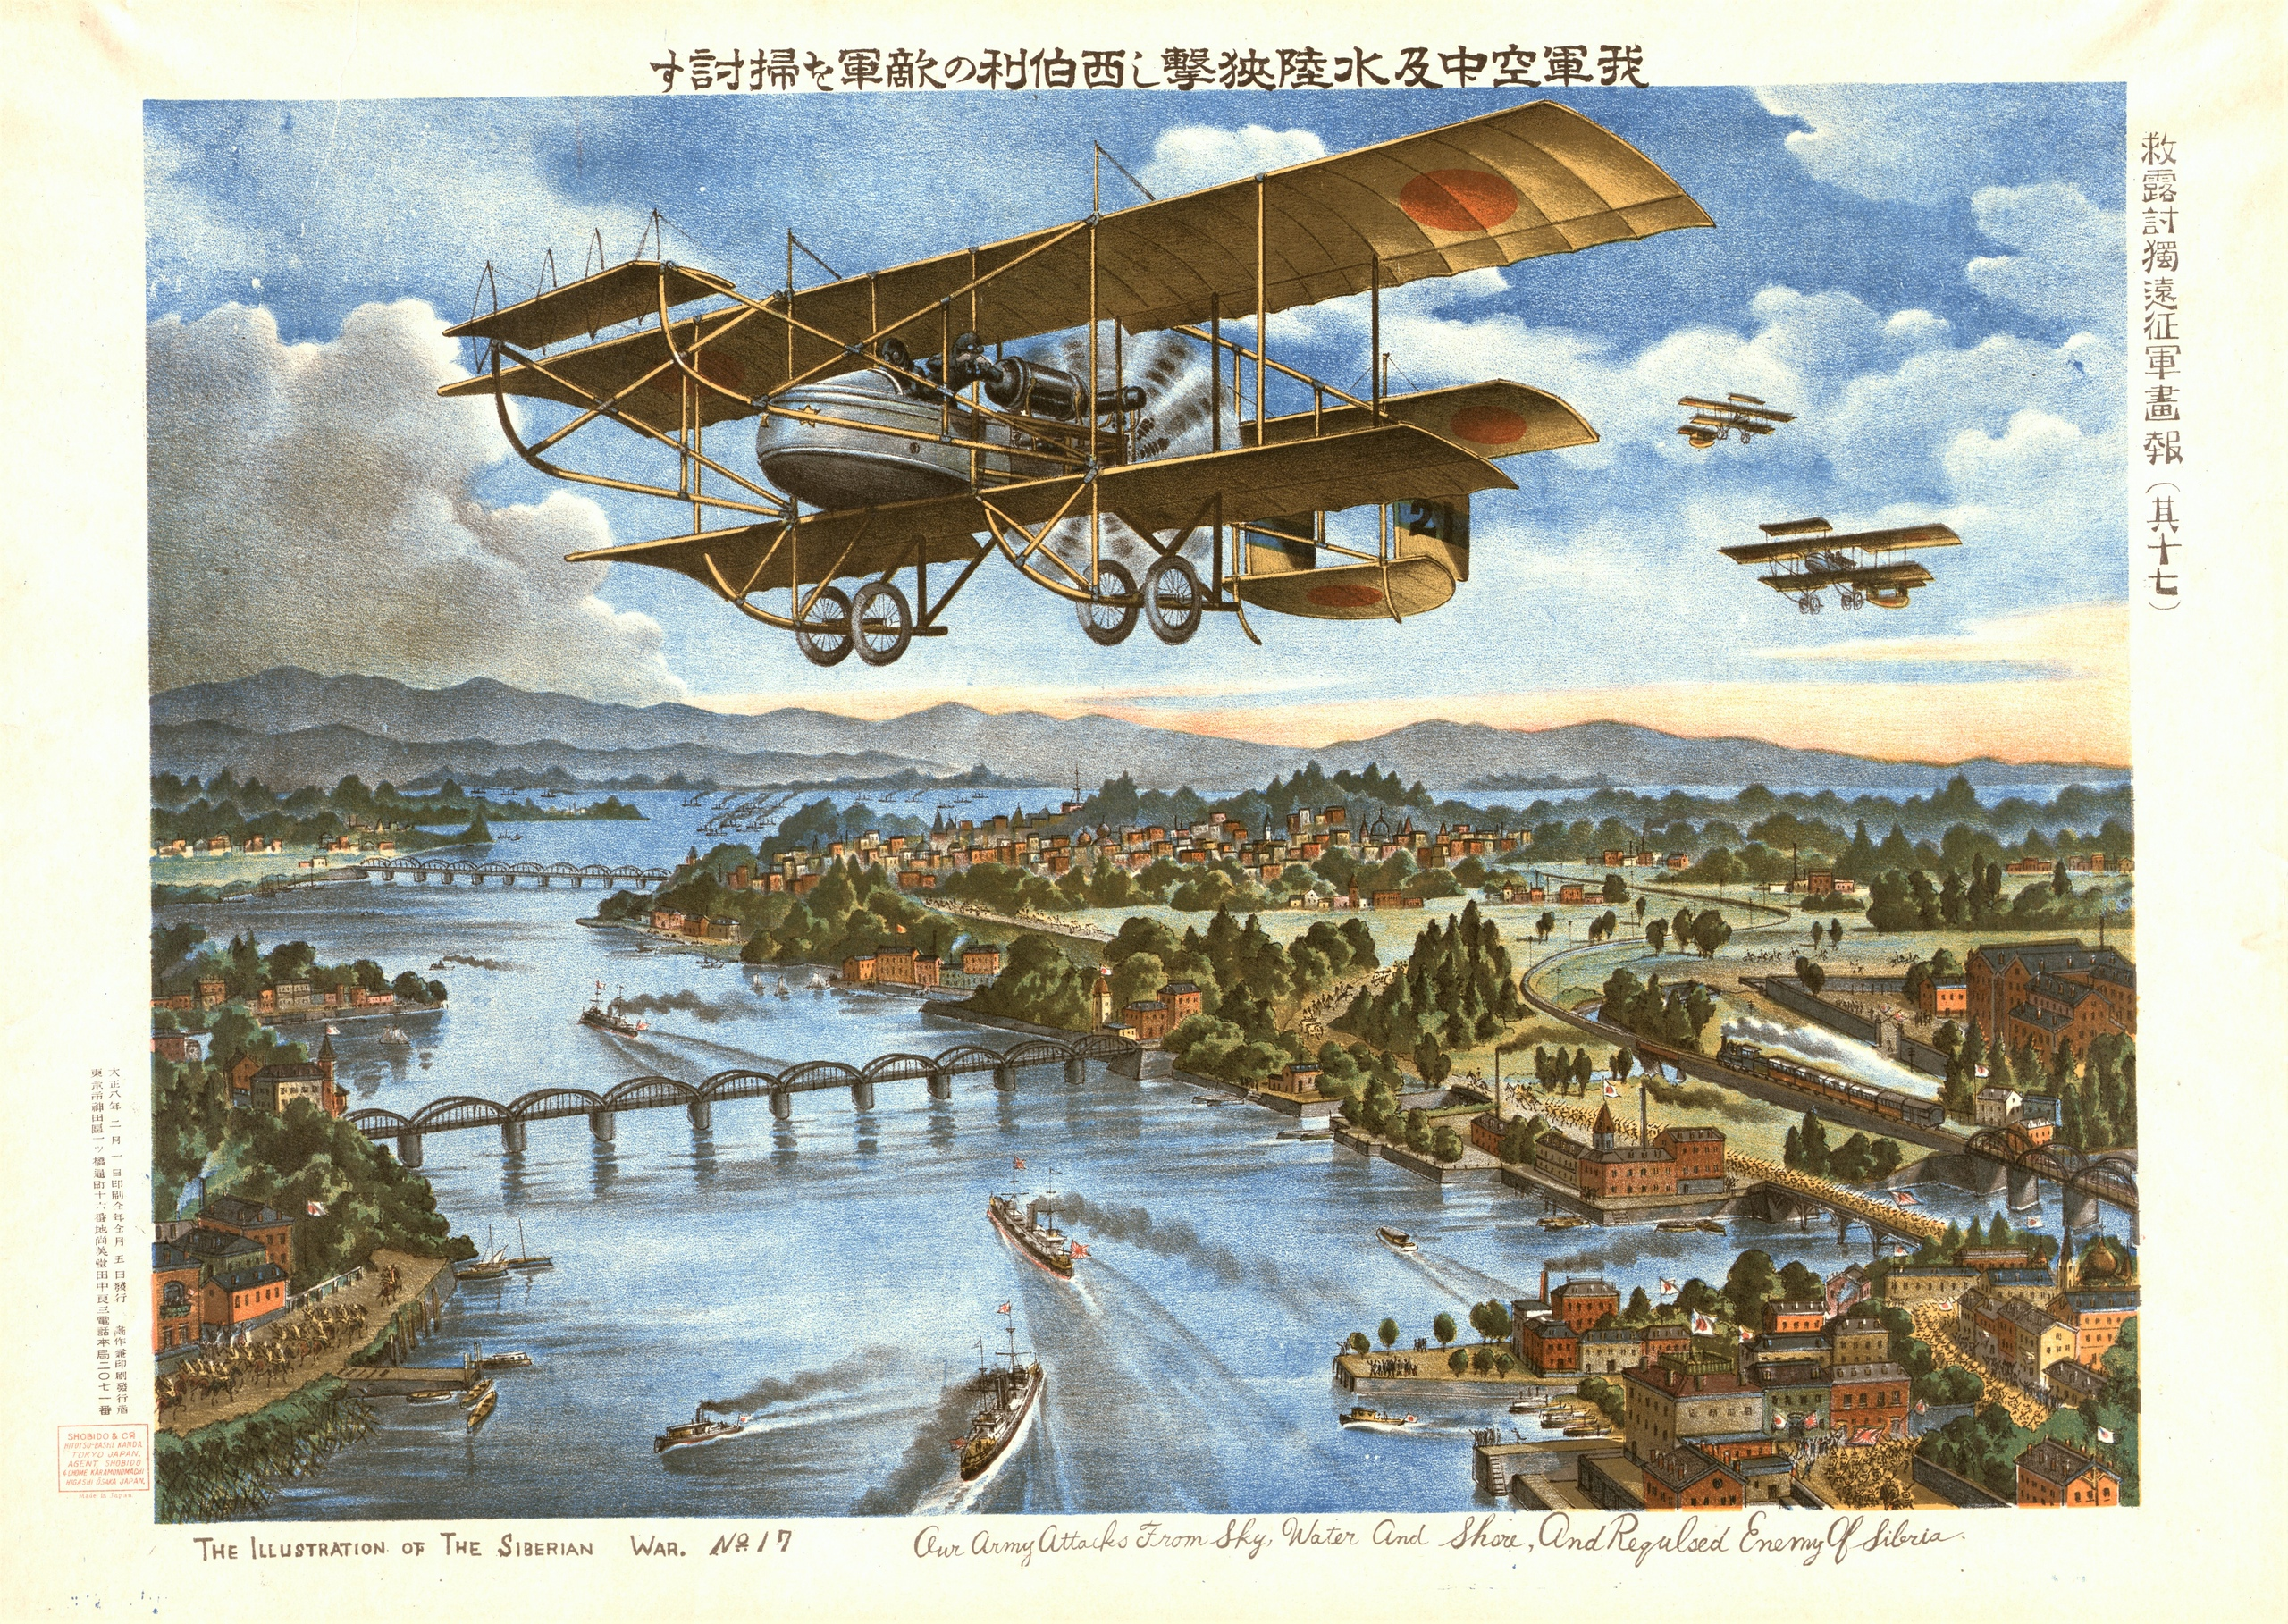
\includegraphics[scale=0.2]{Glava5/lGSk4J5QeZg.jpg}
	%	\label{fig:scipion} % Unique label used for referencing the figure in-text\end{document}
	%	%\addcontentsline{toc}{figure}{Figure \ref{fig:placeholder}} % Uncomment to add the figure to the table of contents%----------------------------------------------------------------------------------------
	\caption{Японский плакат 1918 года, приуроченный к занятию Хабаровска.По самой стилистике видно — здесь планируют остаться надолго.}%	CHAPTER 2
\end{figure}

Полный успех! Блистательная победа! Только вот сам Тераути Масатакэ ко всё тому же октябрю 1918 уже был вынужден подать в отставку со своего поста. Мало того, он вообще оказывается выброшенным из политики, до самой своей, довольно скорой, впрочем (он скончается 3 ноября 1919 года) смерти.

Но почему? Причиной стали Рисовые бунты. И теперь мы поговорим о них подробно. В конце прошлой части было сказано о том, как затягивание Первой Мировой повлияло на глобальный продовольственный рынок и о том, почему это было так важно и болезненно для Страны Восходящего солнца. Уже в 1917 рост цен сказывался достаточно серьёзно и тяжело, а в 1918 положение усугубилось. При этом, как уже было сказано, правительство не приняло никаких мер, которые могли бы смягчить складывающееся положение. Предполагалось, что все многочисленные вложения в назовём его “Китайский проект” начнут, наконец, окупаться. Сам по себе такой подход был достаточно наивен – даже если бы в 1918 это и произошло, то доходы получили бы только представители крупного капитала, которые начали постепенно хозяйственное проникновение в Манчжурию. Со временем расширение сферы экспорта и приток более дешёвого сырья должен был, несомненно, сказаться и на экономике в целом, в том числе и на уровне жизни обычных японцев, но это никак не могло произойти раньше, чем через 3-5 лет. В реальности же вышло следующее. В 1914-1915 годах рядовые жители Японии не ощущали, что с кем-то и за что-то ведётся война, и это было весьма удобно для правительства. В 1918 они уже не понимали, с кем и почему ведётся война, но вполне ощущали её последствия. Русские только что были союзниками, а теперь десятками тысяч на их территорию направляются войска, снаряжаемые, разумеется, не задаром... Обстановка медленно, но верно становилась взрывоопасной. Не доставало толь одного – фитиля, который подожжет пороховой погреб, не доставало зачинщика. В Японии отсутствовали революционные и рабочие партии, которые делали бы ставку на политическую мобилизацию народных масс и действительно серьёзные перемены, вплоть до полного демонтажа сложившейся социально-экономической системы страны. Социал-демократической партии в середине 1900-х не позволили оформиться власти. Коммунистическая партия Японии возникнет только в 1922. Сильные профсоюзы также отсутствовали. Не было и популистов, которые раскачивали бы народ для того, чтобы в дальнейшем шантажировать действующее правительство. Иными словами, не было тех, кто мог бы организовать выступление. Это снижало вероятность того, что оно вообще начнётся, но зато резко осложняло для властей дело, если всё же грянет бунт, потому что он в этом случае выходил бы стихийным, децентрализованным, а потому особенно трудно подавляемым.

Вспыхнуло в небольшом портовом городке Ниси-Хасамати в префектуре Тояма. Причём, в этой истории видны как черты сугубо японского национального колорита, так и весьма занятные параллели и с Великой Французской и с Великой Русской революциями. Итак, основная часть мужчин города занималась рыболовством, причём не каботажным, а на довольно приличном удалении от него – в районе севернее Сахалина и далее в Охотское море. В конце лета 1918 года рыбакам внезапно пошёл очень хороший лов, в связи с чем отцы семейств не спешили возвращаться в город, с тем, чтобы побольше заработать. Действительно, после реализации пойманной рыбы они смогли бы несколько поправить свои дела, вот только до этого момента нужно было ещё дожить тем, кто остался в Ниси-Хасамати. У семей рыболовов стали заканчиваться и запасы пищи, и деньги, которые не давали нормально накопить случайные заработки. Рис – основной продукт питания, уже давно и неуклонно дорожал, и вот теперь сделался ожидающим кормильцев женам и детям не по карману. Видя это, рисоторговцы приняли решение переправить залёживающийся товар в другие, более состоятельные населённые пункты Японии – в порту начали нагружать рисом корабль, который должен был вывезти его из Ниси-Хасамати. При этом данную операцию как-либо скрыть от людей никто не потрудился. В итоге вечером 3 августа 1918 года местные женщины после работы небольшими группами вышли на улицы города. Всего на берегу моря собрались 200—300 женщин, впоследствии образовавших 3 отряда, первый из которых отправился соответственно к дому председателя муниципалитета с требованием прекратить вывоз риса, второй же и третий двинулись к дому торговца рисом, выдвинув требование реализовывать продажу риса лишь местным жителям и по более низкой цене. Нельзя не провести параллелей и с походом парижанок к Версалю, и начавшуюся не когда-нибудь, а в День Работницы, 8 марта по новому стилю Февральскую революцию в Петрограде, где женщины возмутились в хлебных очередях…

Власти Ниси-Хасамати отреагировали жестко. В места скопления женщин была стянута полиция, из-за действий которой многие женщины получили ранения. К ночи прения прекратились, и у рисовых складов были выставлены патрули. Всё? Как бы не так! Слухи разошлись быстро. Аналогичные акции начались на следующий день, 4 августа, в ещё одном похожем рыбацком городе Хигаси-Мидзухаси. Вечером на берегу моря 800 женщин со старшими дочерьми и, что важнее, сыновьями организовали группы по нескольку человек и двинулись в город. Сразу же был дан сигнал полиции, однако она на это раз оказалась беспоиощна против такого числа людей. 5 августа власти, наконец, попытались погасить пожар не силой, а хоть как-то решив проблему: из муниципалитета в Кобе отправили телеграфное сообщение с просьбой выделить определённое количество риса для покрытия дефицита. К тому времени жёны рыбаков устроили себе штаб в местном храме, установили пикеты по всему городу и в близлежащих населённых пунктах с целью проведения слежки за действиями, предпринимаемыми торговцами рисом.

Пока в Кобе думали, бунт вспыхнул и на территории города Намэригава. Причём дополнительным фактором стал следующий – начавшим всё же понемногу возвращаться рыбакам сообщали, что в их отсутствие их женщины оказались избиты полицией. Таким образом, когда к ночи 6 августа к выступлениям подключились и представители мужского пола, в количестве двух тысяч человек организовавшие переговоры с богатым купцом Каном, настроены они были весьма решительно. Пока ещё появление полиции позволяло купировать очаги бунтов, но на следующий день всё повторялось снова и во всё возрастающем масштабе. Власти не могли ни удовлетворить по-настоящему требования протестующих, ни проявить подлинную жесткость и твёрдо подавить любые выступления. Вообще главной проблемой было полное отсутствие у японских управленцев опыта в деле силового ли, мирного ли взаимодействия с чего-то требующими массами. Рисовые бунты, разумеется, не были первыми в истории страны, но почти всегда раньше явно или тайно за всяким мятежом стояли аристократические кланы, даймё, самураи, преследовавшие свои интересы. Здесь же действительно стихийно действовал сам народ. Против любой фронды в старом феодальном духе немедленно направили бы армию, но не расстреливать же из пулемётов рыбачек с детьми, требующими пропитания!? Во всяком случае, в Стране Восходящего солнца до таких вершин прогресса ещё не дошли.

Ещё хуже было с мерами поддержки. Здесь, конечно, властям не повезло, что проблемой стал именно рис. Во-первых, люди здесь не могли и отказывались ждать – в самом деле, голодный желудок не терпит никаких задержек. Во-вторых, если с крупной промышленностью в лице дзайбацу был налажен диалог, и вполне можно было попросить временно чуть снизить цены, пока основная протестная волна не спадёт, то рисовая торговля, особенно итоговый сбыт, находилась в руках множества средних и мелких дельцов, с которыми договориться было никак нельзя. Оставались два варианта. Первый - директивно требовать снижения цен, на что правительство не пошло из страха показать таким образом слабость даже не столько перед мятежниками, сколько, в типично японском духе, слабость перед самой ситуацией – если бы цены всё равно не удалось бы сбить, то получалось бы, что власти не знают, что делать, а это совершенно недопустимая потеря лица. Второй – устраивать рисовые раздачи наиболее нуждающимся, но здесь был риск, затратив государственные средства, лишь пробудить новые аппетиты, не погасив, а подогрев натиск страдающих от дороговизны. Наконец, премьер и его команда сперва до последней крайности не замечали в своих международных играх всей значимости происходящего, а потом оказались в полной растерянности, если не прострации.

В итоге власти Страны Восходящего солнца попали в классическую ловушку полумер. Они оказались бессильны решить проблему, но сумели привлечь к ней всеобщее внимание страны, а перебор разных вариантов выглядел как непоследовательность и даже страх, попытки ухватиться за всякую соломинку. Кое-что было, в самом деле, откровенно глупым. В частности попытки сохранить некую секретность в тот момент, когда в акциях экспроприации зерна принимали участие десятки тысяч людей. Но вернёмся к хронологии. Решающим днём стало 10 августа, когда из портовых городков пламя перекинулось на один из крупнейших городов страны – древнюю столицу – Киото, причём там основной частью протестующих были уже промышленные рабочие. Толпы голодающих открыли рисовые лавки и стали делить рис. 11 -12 августа начались многотысячные выступления городской бедноты в таких городах, как Осака, Кобэ, Нагоя, распространившиеся затем на Токио и другие города. Реакцией на тщетные потуги полиции возвращать на склады разделённую восставшими собственность, стало то, что эти амбары стали просто жечь, ну а после перешли и на дома богачей. 

\begin{figure}[h!tb] 
	\centering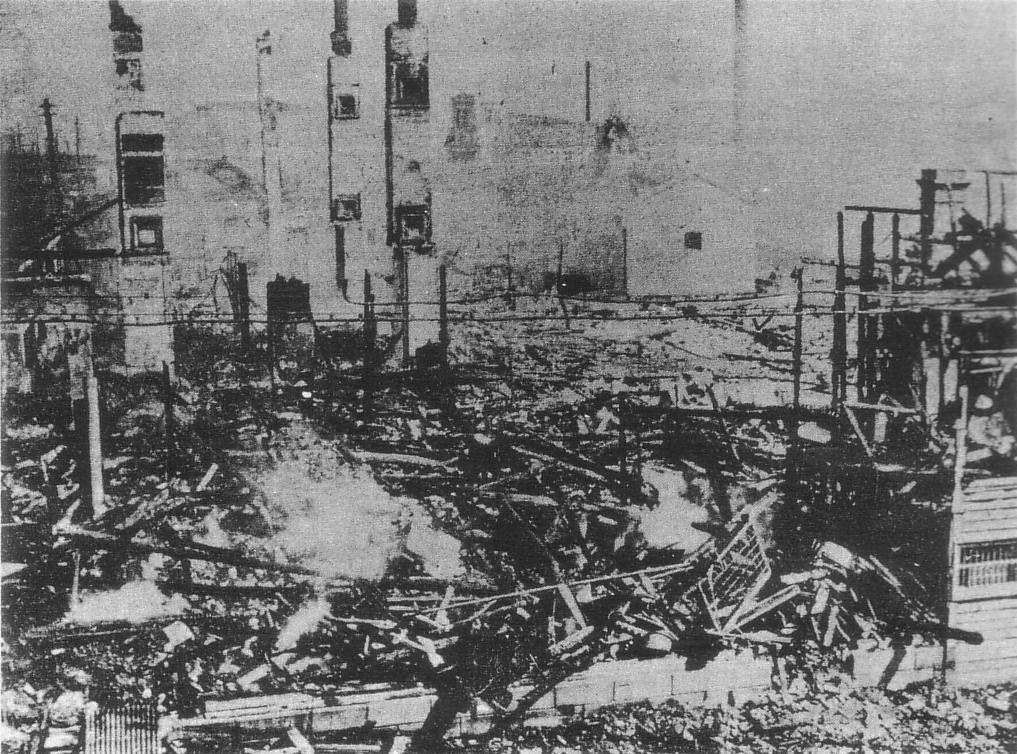
\includegraphics[scale=0.4]{Glava5/L0rhzLzA5u4.jpg}
	%	\label{fig:scipion} % Unique label used for referencing the figure in-text\end{document}
	%	%\addcontentsline{toc}{figure}{Figure \ref{fig:placeholder}} % Uncomment to add the figure to the table of contents%----------------------------------------------------------------------------------------
	\caption{Магазин «Сузуки Сётэн» в Кобе, принадлежавший одноимённой компании, уничтоженный бастующими. 12 августа 1918 года}%	CHAPTER 2
\end{figure}

К концу августа месяца могло показаться, что в стране началась революция: в той или иной форме бунты охватили 36 префектур, или две трети территории государства, общей численностью населения 10 миллионов человек, вообще и 144 города в частности! Теперь уже до 90 \% участников рисовых бунтов являлись рабочими.

\begin{figure}[h!tb] 
	\centering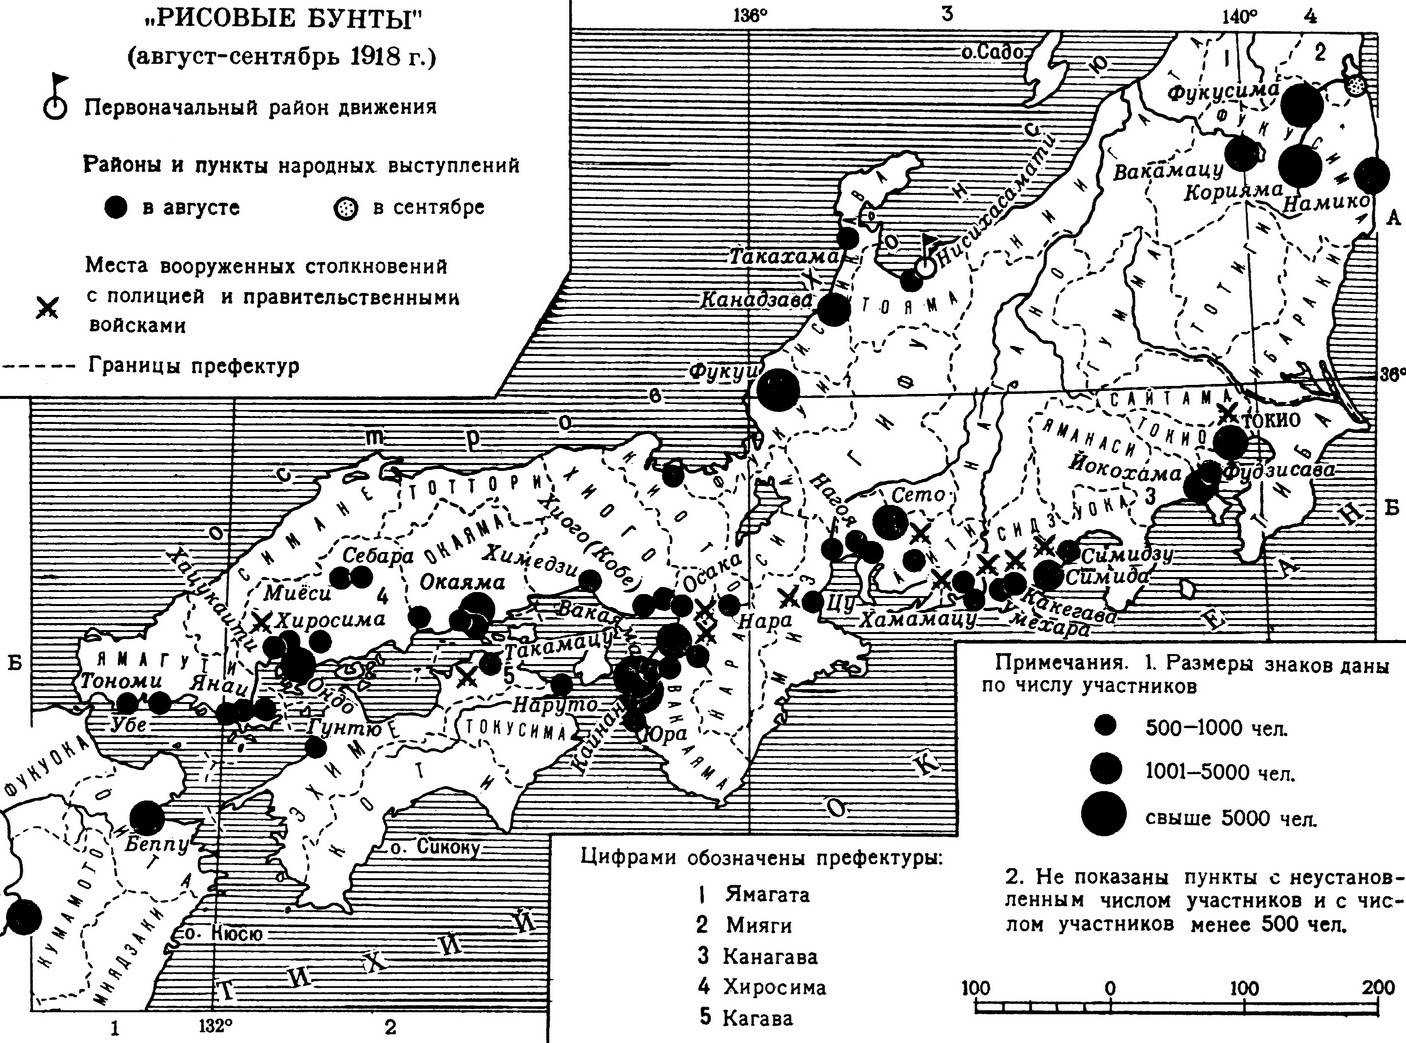
\includegraphics[scale=0.3]{Glava5/obd57lK1104.jpg}
	%	\label{fig:scipion} % Unique label used for referencing the figure in-text\end{document}
	%	%\addcontentsline{toc}{figure}{Figure \ref{fig:placeholder}} % Uncomment to add the figure to the table of contents%----------------------------------------------------------------------------------------
	\caption{Карта Рисовых бунтов}%	CHAPTER 2
\end{figure}

 Будь в Японии даже не то что свои Ленин и РСДРП, а вообще любая социалистическая, или даже бонапартистская партия, готовая решительно взять на себя роль политического лидера – и весь прежний строй полетел бы к чертям. Даже император мог бы не удержаться. Масатакэ не нашёл ничего лучшего, чем активно привлечь к борьбе с повстанцами армию в своём стиле жесткости, решительности и напора. Но тут обнаружилось, что военным оказывают весьма упорное сопротивление, благо местные жители хорошо знали свои города и селения. Было по-прежнему неясно, что вообще происходит: заговор и мятеж неких злодеев – но и солдатам, и даже офицерам понятно, что это не так – хотя бы по той причине, что бунтовщиков слишком много. Гражданская война? Но ни одна из сторон не выдвигала ясно артикулированных политических требований. Война голодных с сытыми – да. И здесь был весьма серьёзный риск, что солдаты прислушаются к собственным животам больше, чем к чему-либо другому, и примкнут к борьбе голодных.

В сентябре 1918 старая государственность Японии повисла на волоске. Большинство мятежников почти наверняка сохраняли лояльность императорской династии, вот только как раз императора, способного призвать страну к миру, не было – был больной Тайсё. Масатакэ утратил контроль над ситуацией. В дело экстренно вмешиваются Гэнро – к этому моменту их остаётся трое: Ямагата Аритомо, Мацуката Масаёси и Сайондзи Киммоти. Действуя в ручном режиме они должны были буквально за две-три недели погасить разверзшееся инферно кризиса, решив сложнейшую задачу, а именно восстановление полноценной связи, контакта между управляющими и управляемыми, доверия народа если даже не ко всей власти, то к какой-то части системы, используя которую можно будет начать переговоры, вбрасывать в массы те или иные предложения. При этом все традиционные центры силы отпадали. Император, сами Гэнро, бюрократия с устойчивым запахом пороха, идущим даже и от деловых костюмов – всё не то. Оставался лишь парламент. Маркиз Сайондзи экстренно проводит переговоры с лидером крупнейшей фракции а в прошлом журналистом и дипломатом Хара Такаси. 

\begin{figure}[h!tb] 
	\centering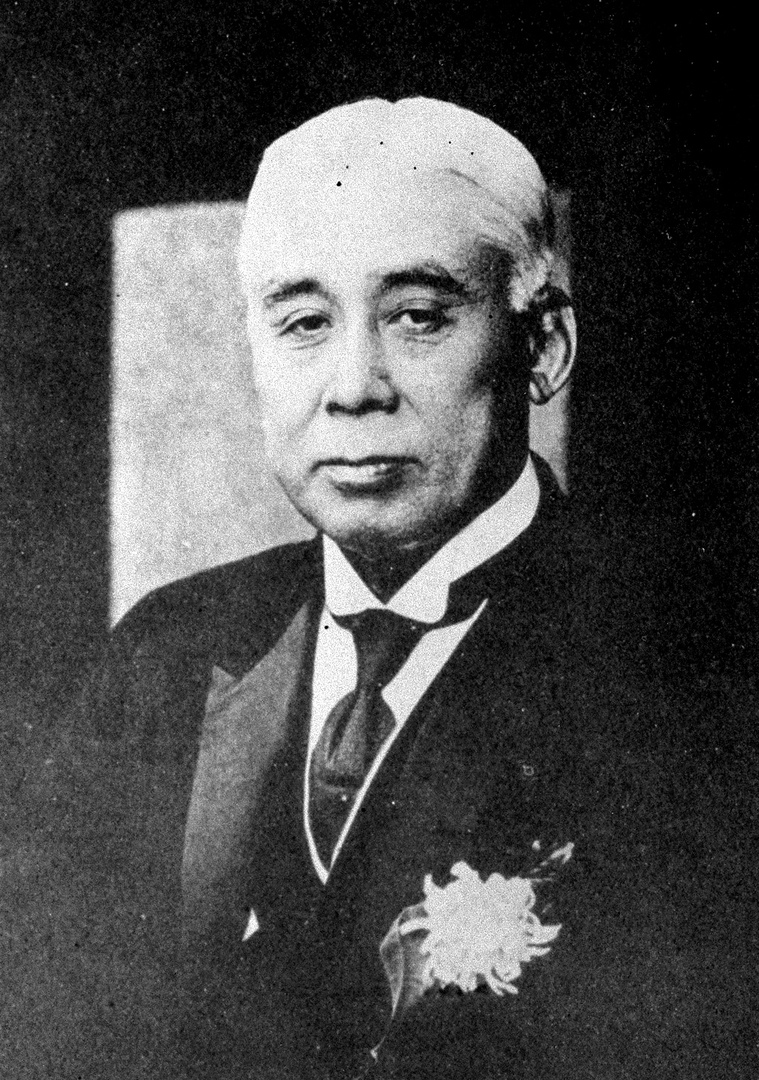
\includegraphics[scale=0.4]{Glava5/dY0QHkyaOvM.jpg}
	%	\label{fig:scipion} % Unique label used for referencing the figure in-text\end{document}
	%	%\addcontentsline{toc}{figure}{Figure \ref{fig:placeholder}} % Uncomment to add the figure to the table of contents%----------------------------------------------------------------------------------------
	\caption{Хара Такаси}%	CHAPTER 2
\end{figure}

Его партия Риккэн Сэйюкай, или Друзья конституционного правительства была куда теснее связана с капитанами дзайбацу, особенно с группой Мицуи, а не с рабочими и рыбаками, но особенного выбора не было. Сайондзи даёт партии и её лидеру карт-бланш, впервые в истории страны они получают возможность сформировать правительство парламентского большинства, не являющее ответственным министерством по букве закона, но фактически бывшее таковым и работающее в тесной связке с депутатами. Маркиз и остальные Гэнро ради этого даже ломают с хрустом карьеру и судьбу некогда весьма полезного Масатакэ – как уже было сказано, 29 сентября 1918 его убирают с поста премьера вместе со всей командой. Члены партии Риккэн Сэйюкай назначаются на должности всех министров, кроме министра по делам армии, министра по делам флота и министра иностранных дел. Партия получает поддержку и финансирование. В обмен на это нужно лишь одно – установление надёжного контакта хотя бы с частью тех, кто разносит полицейские участки и склады, возвращение их в легальный политический процесс и в дальнейшем борьба с протестными настояниями уже не одними только полицейскими дубинками, а партийно-политической пропагандой. Иными словами, Друзья конституционного правительства должны были, став первой в истории Страны Восходящего солнца правящей партией, создать какой-никакой социальный лифт помимо армии, а главное – отделить в народном движении буйных от конструктивных.

В общем и целом план удался. Крупные политические перемены смогли заставить часть ведущих борьбу масс поверить, что они одержали победу и теперь могут уже без риска и в рамках закона оказывать влияние на принимаемые наверху решения. С остальными же теперь не церемонились. Порядка 8000 человек, выявленных в качестве зачинщиков и лидеров, было арестовано. 7813 из них по итогам судебных заседаний были приговорены к разным срокам лишения свободы. Маркиз Сайондзи в 1920 году станет герцогом (или князем, или, по-японски косяку). 

\begin{figure}[h!tb] 
	\centering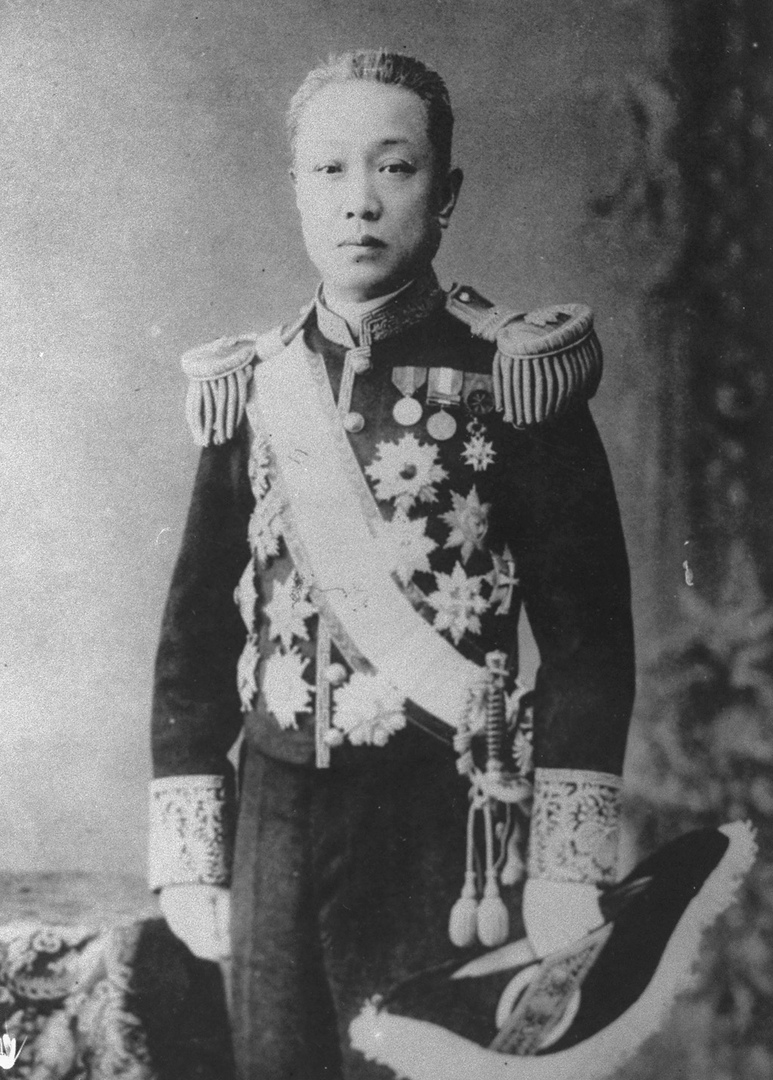
\includegraphics[scale=0.4]{Glava5/ESDTnoAPRIc.jpg}
	%	\label{fig:scipion} % Unique label used for referencing the figure in-text\end{document}
	%	%\addcontentsline{toc}{figure}{Figure \ref{fig:placeholder}} % Uncomment to add the figure to the table of contents%----------------------------------------------------------------------------------------
	\caption{Сайондзи Киммоти, герцог, гэнро и просто человек, очень много сделавший для Японии}%	CHAPTER 2
\end{figure}

Рисовые бунты окончатся. Японская империя устоит. Вот только в мире за то время, которое Япония была вынуждена сконцентрироваться на внутренней политике, многое успело измениться. В начале августа 1918 провалом окончилось последнее крупное немецкое наступление на Западном фронте – 2-я битва на Марне. С этого момента инициатива перешла в руки Антанты, что давало ей возможность куда эффективнее реализовывать имеющееся превосходство в силах и средствах. 8 августа уже они начали так называемое Стодневное наступление, в ходе которого немецкие армии были почти полностью вытеснены с захваченных территорий Франции и частично – Бельгии. Наконец, в ноябре 1918 в Германии начались революционные выступления. Сам фронт ещё не рухнул (хотя стратегически положение немцев было уже совершенно безнадёжным), но рухнуло всё, что было позади него. Отрёкся и бежал император Вльгельм II. 11 ноября 1918 было подписано завершившее Первую Мировую Компьенское перемирие. И только к этому же, примерно, времени, Японии удалось купировать последствия своего внутреннего кризиса.

Окончание Первой Мировой меняло всё. Оно меняло самые цели и смысл Интервенции в России: если прежде основной задачей было, как максимум, воссоздать при любой готовой на это пойти русской власти Восточный фронт, а как минимум не дать Центральным державам возможности воспользоваться ресурсами России для продолжения войны, то теперь речь шла о походе против Великой Русской революции, пока её последствия ещё не приобрели глобальный характер. Оно меняло положение Японии: если прежде малая степень реального её участия в боевых действиях была огромным плюсом, оставляла свободными руки, позволяла с минимальной оглядкой на позицию других держав действовать в Китае и на Дальнем Востоке, то теперь, когда настал черёд подведения итогов и дележа лежащего у их ног мира между победителями, она стала большим минусом. Наконец, пропало, причём разом для внешнего и внутреннего потребителя, оправдание всё большей милитаризации Империи Восходящего солнца.

За 1918 год японские войска добились в России довольно многого, но японская дипломатия, японское государственное руководство оказалось неспособно (в первую очередь из-за радикальных пертурбаций в системе власти, вызванных Рисовыми бунтами) даже частично закрепить и оформить эти успехи. Высадившиеся во Владивостоке части сумели предохранить от разложения, как от пропаганды русских агитаторов, так и от новостей из дома, так что все 72 000 были вполне боеспособными. Со строго военной точки зрения, как скоро убедились японские командиры, этого было вполне достаточно для завоевания всего Дальнего Востока, причём достаточно быстрого и лёгкого. Но действовать этим, наиболее рациональным способом было нельзя по политическим мотивам – и для русских, и для союзников по Антанте происходящее не должно было выглядеть как вторая Русско-японская война. В этом смысле японцы и в 1918 и далее действовали мудрее и осторожнее, чем, например, поляки во главе с Пилсудским, которые из-за этого едва не потеряли всё, в том числе и свежеобретённую независимость. Экспедиционный корпус Империи Восходящего солнца в итоге пришёл к следующей схеме – продвижение вперёд осуществляется силами готовых к сотрудничеству русских боевых отрядов, но сразу за ними следуют уже кадровые японские части, наводняющие и надёжно удерживающие взятый район. Схожим образом старались действовать и иные интервенты. Единственной проблемой в этом варианте было то, что японцы, в отличие от остальных, намеревались закрепить за собой большую часть контролируемых территорий, а раз так, то им следовало избегать установления там системы власти, ориентированной на какую-либо из крупных фракций в Гражданской войне в России, имевших виды на полную победу. В первую очередь, конечно, речь идёт о Колчаке. Автор предупреждает, что сейчас его может понести, но постарается сдержаться, благо формат серии и объём статьи не позволяют особенно разойтись. Вкратце: из большого количества, благо единством они никогда не отличались, руководителей Белого и антибольшевистского движения Колчак – наиболее явная и наиболее значимая креатура внешних игроков, Антанты и, в первую голову, Британии. Свидетельств тому много – начиная от полушутливых, но весьма широко ходивших строк, вроде:

“Мундир английский,

Погон французский,

Табак японский,

Правитель омский”.

и вплоть до мест в воспоминаниях самих белых деятелей, в частности Деникина и других руководителей Добрармии, где весьма ясно видно, как активно, доводя едва не до шантажа, зарубежные “друзья” вынуждали его признать хоть номинально главенство адмирала.

Общеизвестный факт вполне официальный переход Колчака на службу королю Георгу V, несколько меньше определённости в том, как он взаимодействовал с американцами, однако к моменту его возвращения из-за границы в Россию через уже занятый интервентами Владивосток (к слову, в процессе побывал Колчак и в Японии, где даже имел встречу с начальником японского Генштаба генералом Ихарой и его помощником генералом Танакой, впрочем, оставшимися недовольными гостем), между главными странами Антанты уже существовал консенсус – это тот человек, который готов проводить устраивающую их политику и которому они в свою очередь готовы оказывать полную поддержку. Как частное лицо, Колчак едет через Сибирь – вроде бы как на Дон (хотя прямая связь к этому моменту уже отсутствует), опять же, вроде бы как, только на несколько дней останавливается в Омске. Было это 13 октября 1918. А уже 16 октября генерал Болдырев от имени Директории предложил Колчаку пост военного и морского министра. Вот просто так, потому что гладиолус – я напомню, что у адмирала нет никакого опыта командования сухопутными силами, он не является лидером или даже просто членом какой-либо партии, он вообще только недавно, повторю, возвратился на родину. Причём Колчак ещё сперва отказывается, выторговывая себе особые условия – и Директория принимает и их - 5 ноября 1918 года адмирал назначен военным и морским министром Временного Всероссийского Правительства. Но им Колчак пробудет недолго. 11 ноября 1918 оканчивается Первая мировая, а ровно неделю спустя лучший друг Британии и вообще Антанты Колчак совершает натуральный государственный переворот, свергает руководившую Сибирью Директорию и становится диктатором с наскоро придуманным титулом Верховного правителя России. Как всё это стало возможно? За счёт чего? Не нужно быть семи пядей во лбу, чтобы понять это.

Колчак, как было сказано выше, устраивал лидеров Антанты: Британию, США, Францию. Но только не Японию. Адмирал строил власть, хотя реально и зависимую от воли победителей Первой мировой, но, всё же, номинально суверенную. Японцам же был нужен тот, кто будет махать шашкой, не особенно задумываясь о будущем статусе того, что будет ею взято. И такой человек нашёлся - атаман Семёнов - человек лихой, амбициозный, но абсолютно не способный к политическим, а не сугубо военно-силовым методам руководства.

\begin{figure}[h!tb] 
	\centering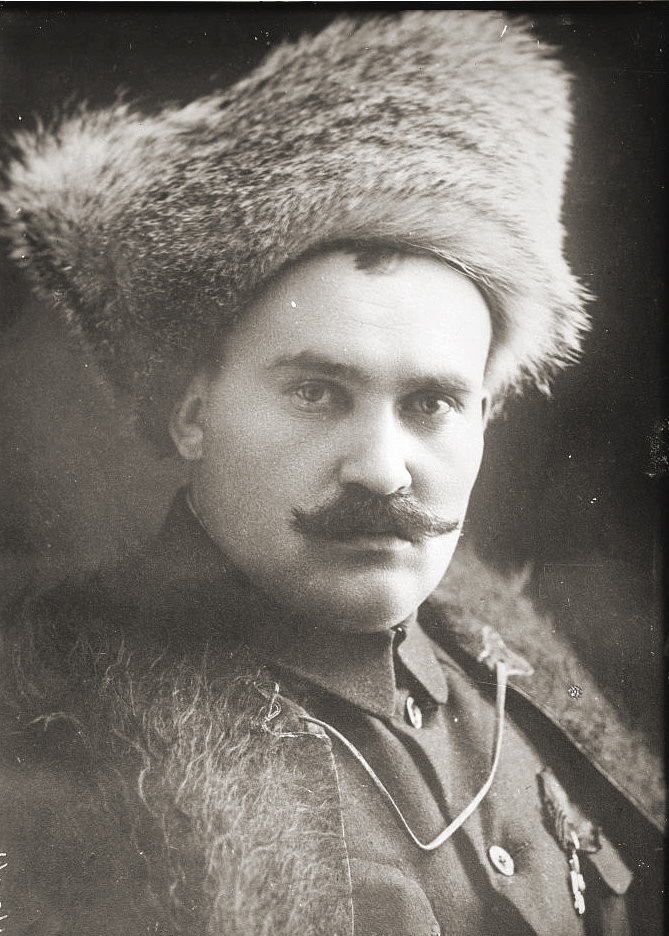
\includegraphics[scale=0.4]{Glava5/H-CriBMSs0Y.jpg}
	%	\label{fig:scipion} % Unique label used for referencing the figure in-text\end{document}
	%	%\addcontentsline{toc}{figure}{Figure \ref{fig:placeholder}} % Uncomment to add the figure to the table of contents%----------------------------------------------------------------------------------------
	\caption{Атаман Семёнов}%	CHAPTER 2
\end{figure}

Под его руководством был сформирован так называемый Особый Маньчжурский Отряд, фактически превратившийся к середине 1918 в его личную банду. Эти силы и послужили интересам Империи Восходящего солнца. В наступлении на Читу в августе 1918 года ОМО Семенова непосредственно поддержала Сводная бригада Японской императорской армии под командованием генерал-лейтенанта Фудзия. 6 сентября 1918 года объединенный авангард ОМО и японских войск вступил в Читу. Третья дивизия императорской армии после захвата Читы выделила из своего состава отряд генерал-майора Юхары для оккупации Амурской железной дороги, которая к 12 сентября была полностью очищена от красных и вообще от всех, кто мог сопротивляться японцам. К 20 сентября 1918 года отряд Фудзии был отозван из Забайкалья, но скоро сменён - охрану железной дороги взяли на себя подразделения Третьей дивизии императорской армии. Ещё позднее её сменила пятая дивизия генерала Судзуки.

Отношения с Колчаком у Семёнова, а главное у японцев были… противоречивые. Ещё при Директории атаман легализовался - приказом по Сибирской армии от 10 сентября 1918 года Семёнов был назначен командиром 5-го Приамурского армейского корпуса. Однако после переворота 18 ноября 1918 года он первоначально не признал Колчака Верховным правителем, за что приказом от 1 декабря того же года был снят с должности. 8 декабря Семёнов фактически без чьей-либо санкции создал под своим командованием Отдельную Восточно-Сибирскую армию в составе 1-го Отдельного Восточного казачьего, 5-го Приамурского и Туземного конного корпусов. Исполняющим должность начальника штаба армии был назначен полковник Л. В. Вериго. Разумеется, истинными инициаторами были японцы. Колчаку было во-первых не до Семёнова, а во-вторых тот, так или иначе, боролся с красными партизанами и повстанцами, так что в итоге политес был соблюден, Верховный правитель и атаман друг друга таки признали, но фактически Семёнов по-прежнему оставался сам по себе. Численность его “армии” к весне 1919 года составила от 8 до 10 тыс. человек, включая до 5 тыс. забайкальских казаков. Впрочем, её создание так и не было признано Колчаком, так что войско это оказалось на самопрокорме. 9 мая 1919 года третьим Войсковым кругом Семёнов избран войсковым атаманом Забайкальского казачьего войска. По соглашению с атаманами Амурским и Уссурийским он принял должность Походного атамана Забайкальцев, Амурцев и Уссурийцев со штабом на станции Даурия Забайкальской железной дороги, иными словами стала очевидной перспектива полного обособления контролируемой семёновцами зоны в отдельное квазигосударство. В этой ситуации Колчак счёл за лучшее опять сделать шаг навстречу: приказом Верховного правителя от 25 мая 1919 года № 136 Г. М. Семёнов был назначен командиром 6-го Восточно-Сибирского армейского корпуса, в который по приказу Колчака № 470 была переформирована Отдельная Восточно-Сибирская армия. Корпуса, ранее в неё входившие, стали дивизиями. 18 июля 1919 Семёнов был назначен помощником главного начальника Приамурского края и помощником командующего войсками Приамурского военного округа с производством в генерал-майоры, 23 декабря — командующим войсками Иркутского, Забайкальского и Приамурского военных округов на правах главнокомандующего армиями с производством в генерал-лейтенанты. При этом все прекрасно понимали кто такие Семёнов и ряд других ему подобных лиц на самом деле. Ещё в октябре 1918 года помощник генерала Д. Л. Хорвата по военным вопросам генерал П. П. Иванов-Ринов телеграфировал начальнику штаба верховного главнокомандующего Сибирской армией:

«Положение на Дальнем Востоке таково: Хабаровск, Нижний Амур и железная дорога Хабаровск — Никольск заняты атаманом Калмыковым, которого поддерживают японцы, за что Калмыков предоставляет им расхищать неисчислимые ценности Хабаровска. Японцы в свою очередь предоставляют Калмыкову открыто разбойничать, именно: разграбить хабаровский банк, расстреливать всех, кого захочет, смещать и назначать начальников окружных управлений Хабаровска и осуществлять самую дикую диктатуру. Семёнов, поддерживаемый также японцами, хотя и заявляет о своей лояльности в отношении командного состава и правительства, позволяет своим бандам также бесчинствовать в Забайкалье, именно: реквизировать наши продовольственные грузы, продавать их спекулянтам, а деньги делить между чинами отрядов».

Едва ли японские военные-кадровики могли действительно хорошо относиться к этому разбойнику, но использовали Семёнова по полной. Собственно, окончится путь атамана через много лет в 1945 арестом его в Манчжурии. Однако, оставим в стороне эту, конечно, примечательную персону и вернёмся к Империи Восходящего солнца. С одной стороны, к началу 1919 достигнуто было очень многое. И в отношении объема захваченного и в отношении лёгкости, с которой это было сделано. Но было и две серьёзные проблемы. Первая – во Владивостоке продолжали находиться войска других держав Антанты, а прежде всего США. Они и близко не имели того влияния, которое имели японцы, очень сильно уступали им численно, но вот избавиться от их присутствия, делающего все захваты с формальной точки зрения не собственно японскими, а общесоюзными, было решительно невозможно. Вторая – ни Колчак, ни какой-либо другой хоть немного легитимный и чем-то управляющий русский руководитель или орган не легализовал и не закрепил ни пяди дальневосточной и сибирской земли за Японией.

Всё вело к тому, что окончательное решение будет приниматься там, куда в это время съезжался и смотрел с надеждой или страхом весь Земной шар – на мирной конференции в Париже. Она началась 18 января 1919 года. Разумеется, была там представлена и Япония – и не просто представлена: сознавая важность стоящих перед представителем страны задач, во Францию был направлен ведущий из трёх Гэнро, человек, принимавший ключевые решения в период Рисовых бунтов – маркиз Сайондзи Киммоти. И не зря. Настал момент, когда старой китайской хитрости, карте формального участия Поднебесной в войне на стороне Антанты надлежало сыграть или не сыграть свою роль. Китайский представитель Гу Вэйцзюнь, имевший неплохой дипломатический опыт и связи – с 1915 по 1919 год он был послом Китая в США, поднял так называемый Шаньдунский вопрос. Он настаивал на том, что факт присоединения Китая к Антанте обязывает Японию передать пекинскому правительству полуостров Шаньдун, территорию, арендованную Германией и взятую в тот период, когда немцы ещё не были военными противниками Поднебесной. Впрочем, Циндао с окрестностями был лишь предлогом. Фактически же китайцы попытались торпедировать всю систему неравноправных договоров, а в первую очередь принятые ими 16 пунктов. Конечно, говорить, что Китай сыграл сколь либо заметную роль в победе Антанты в первой мировой было бы смехотворно, но, в общем то, Япония здесь не сильно отличалась от него. Весь вопрос был в том, даёт ли японцам тот факт, что их страна присоединилась к борьбе раньше, какие-либо преимущества при заключении мира по сравнению с Китаем. Гу Вэйцзюнь мог считать этот аргумент достаточно сильным, так как не кто-нибудь, а Соединённые Штаты, вступили в войну ближе к её завершению. Но… Реальная политика оказалась сильнее и высоких идей и слов, и международно-правовых установлений. Статья 156 Версальского договора гласила, что Германская империя отказывается от прав на Шаньдун не в пользу Китая, а в пользу Японии. Сохраняли силу и 16 пунктов. Сайондзи смог отстоять то главное, что было основой национальных интересов Империи во внешней политике – завоевания и достижения в Поднебесной. 

\begin{figure}[h!tb] 
	\centering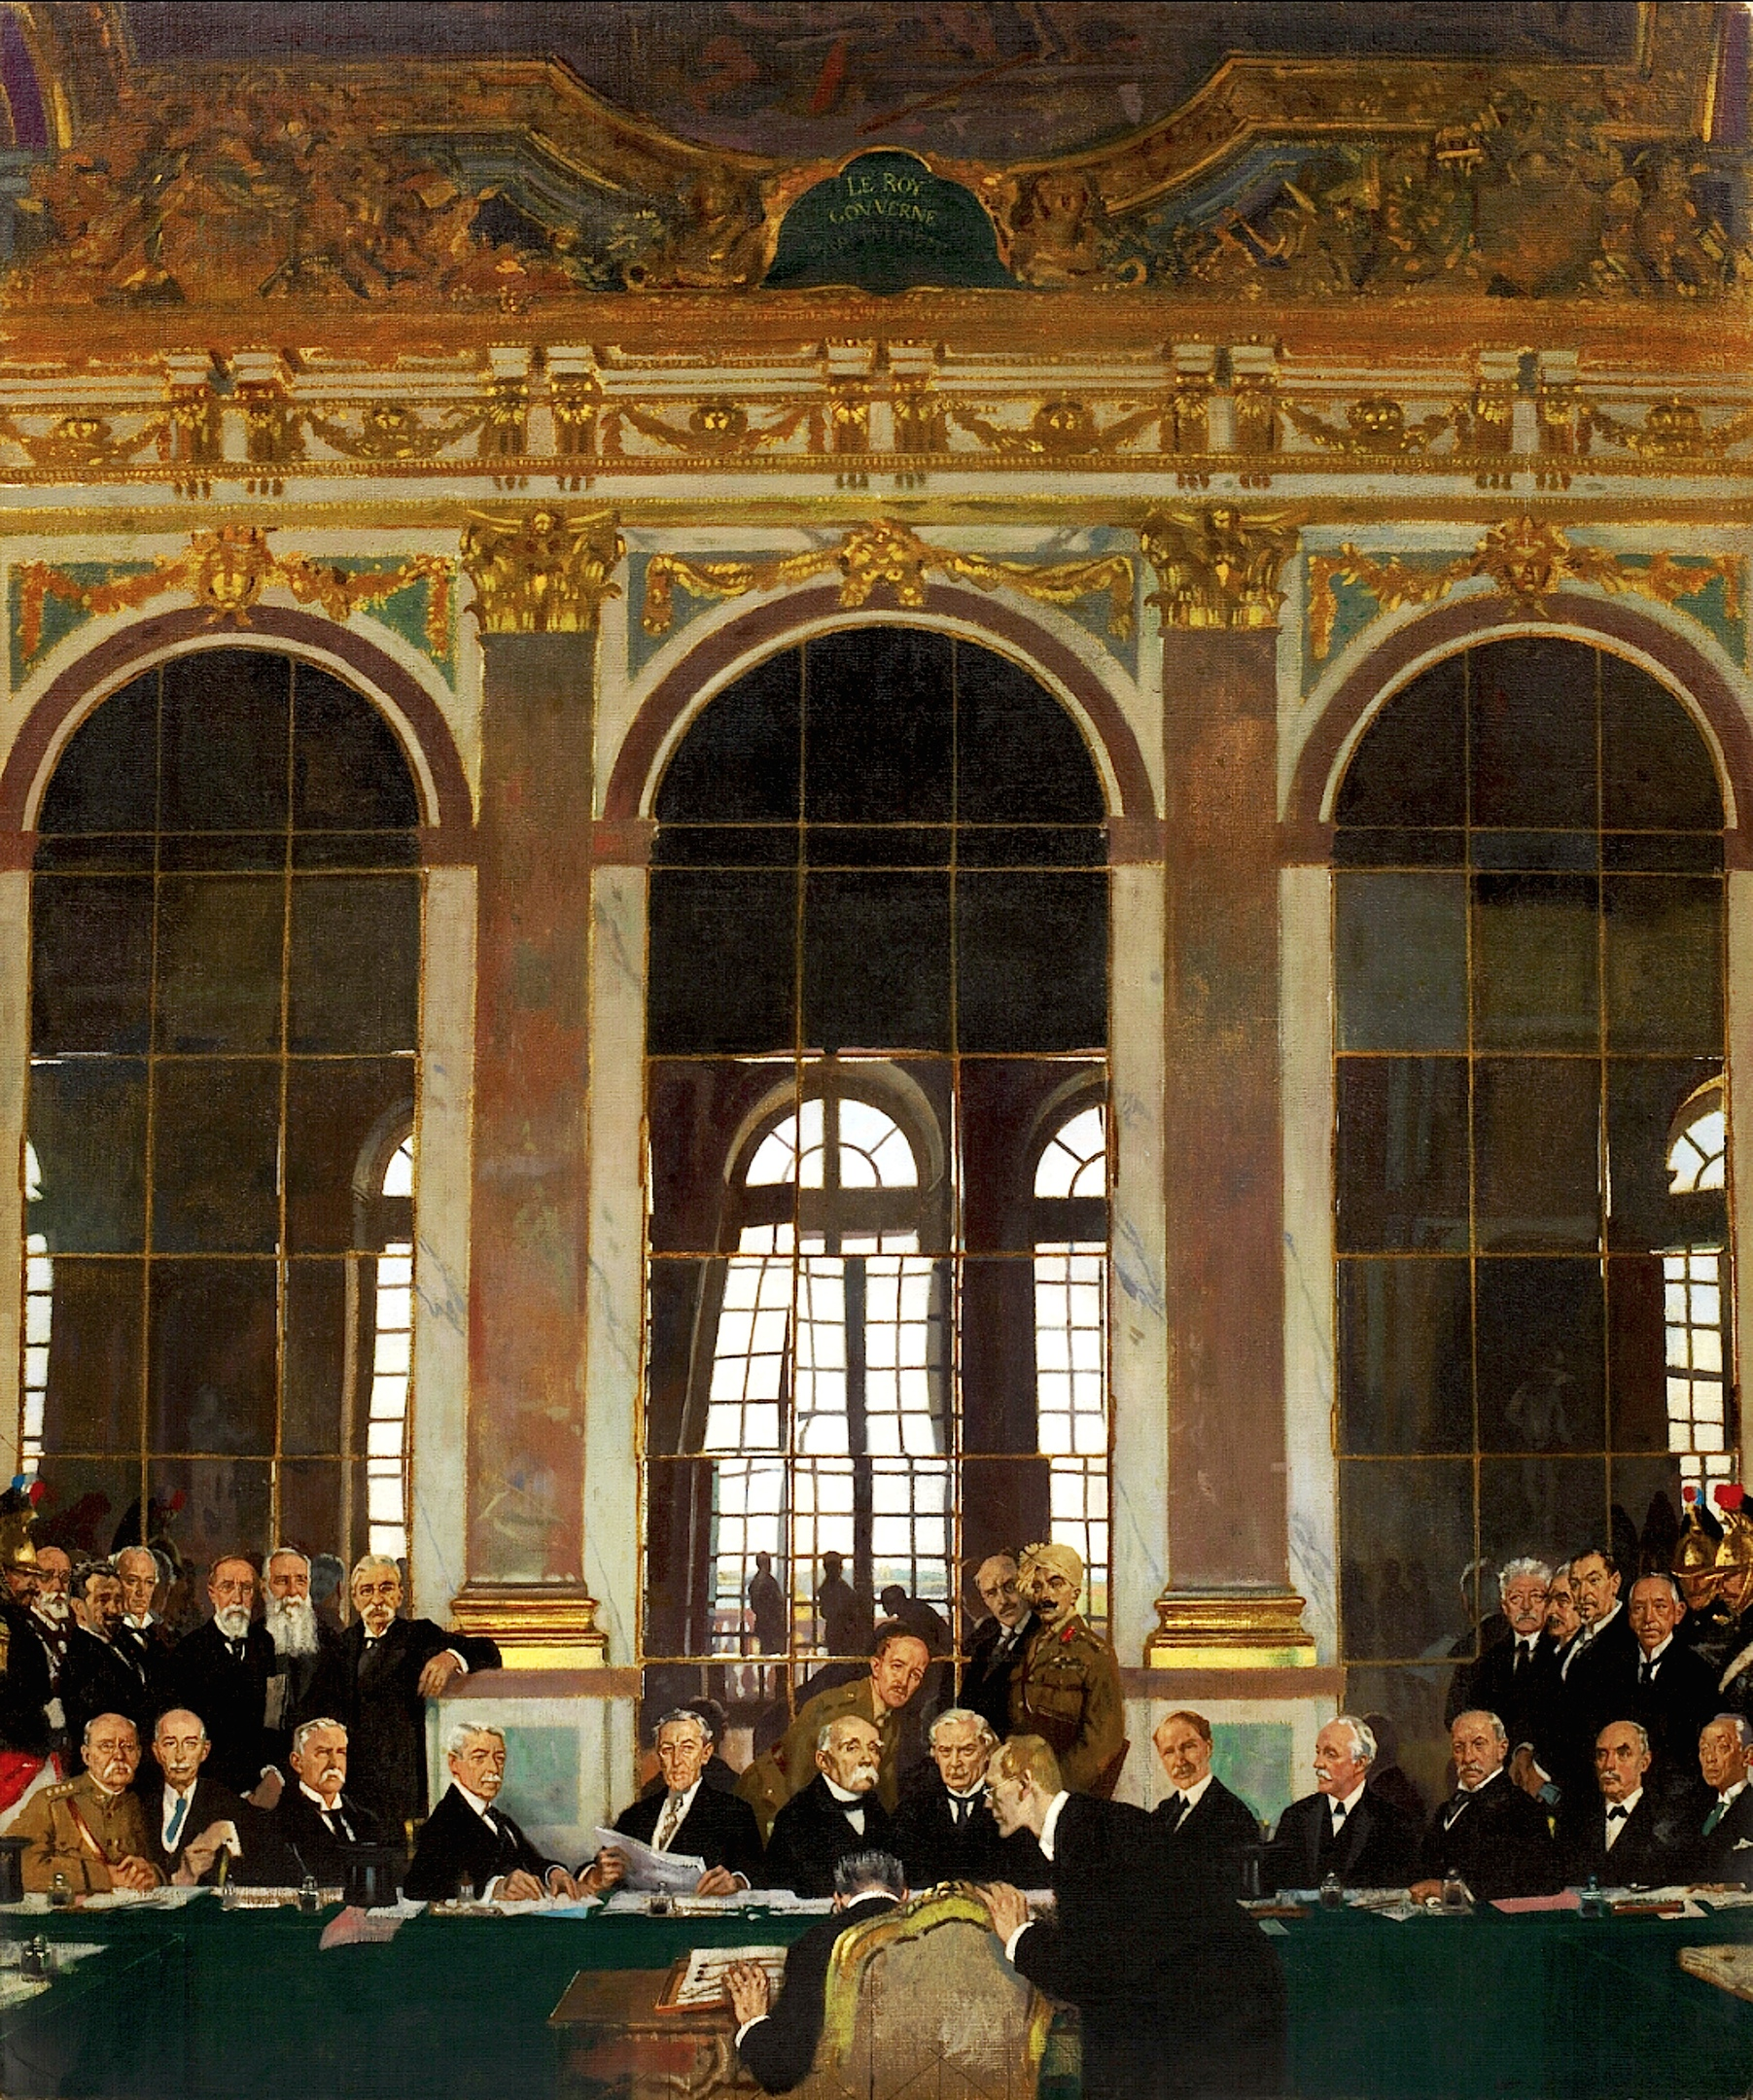
\includegraphics[scale=0.2]{Glava5/1FCWB_wh8ZY.jpg}
	%	\label{fig:scipion} % Unique label used for referencing the figure in-text\end{document}
	%	%\addcontentsline{toc}{figure}{Figure \ref{fig:placeholder}} % Uncomment to add the figure to the table of contents%----------------------------------------------------------------------------------------
	\caption{Подписание Версальского договора. Сайондзи Киммоти — крайний сидящий справа}%	CHAPTER 2
\end{figure}

Но, судя по всему, потому что ни в каких договорах мы этого не найдём, а содержание частных бесед теперь уже точно не восстановишь, в обмен глава японской делегации пообещал, что каких-либо односторонних действий в России вне рамок общей политики победителей его страна предпринимать не будет.

Китайцы демонстративно отказались подписывать Версальский договор, заключив с Германией сепаратный. В стране начались массовые выступления – многие тысячи людей негодовали из-за национального унижения. Японцы могли взирать на это свысока и не без чувства превосходства. Они не знали, что пройдёт совсем немного времени, и им будет суждено испытать всё то же самое и даже больше, но не в Париже, а в Вашингтоне. Но об этом – в следующий раз.

\url{https://vk.com/wall-162479647_83473}